\subsection{I-V Characteristics}
\label{sec:test:iv}

% \hl{6.25\%
%
% Plot the forward and reverse bias VI characteristics of one of your diodes. Describe the salient features of the graphs [150 words max + Figures]}

\begin{figure}[!htb]
  \centering
  \begin{subfigure}[t]{0.5\textwidth}
      % \begin{figure}[!htb]
\begin{center}
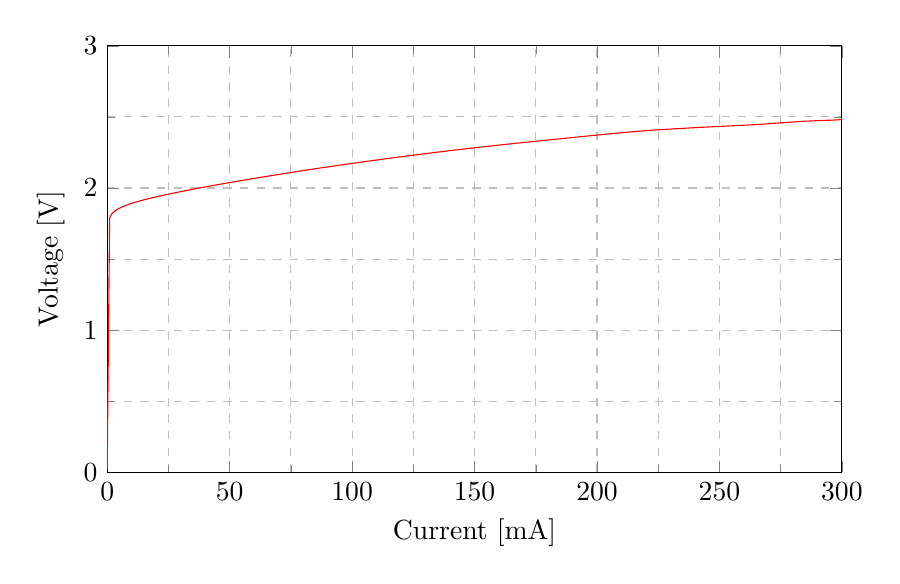
\begin{tikzpicture}

\begin{axis}[
    %title={Temperature dependence of CuSO$_4\cdot$5H$_2$O solubility},
    xlabel={Current [mA]},
    ylabel={Voltage [V]},
    height=7cm,
    width=0.9\textwidth,
    xmin=0, xmax=300,
    ymin=0, ymax=3,
    xtick={0, 50, 100, 150, 200, 250, 300},
    ytick={0, 1, 2, 3},
    legend pos=south east,
    ymajorgrids=true,
    yminorgrids=true,
    xmajorgrids=true,
    xminorgrids=true,
    minor tick num=1,
    grid style=dashed,
]

\addplot[color=red]
  coordinates {
  (0,0.01416543)
  (1,1.791197)
  (2,1.820639)
  (3,1.836875)
  (4,1.84871)
  (5,1.858317)
  (6,1.866541)
  (7,1.873795)
  (8,1.880448)
  (9,1.886535)
  (10,1.892227)
  (11,1.897612)
  (12,1.902734)
  (13,1.907621)
  (14,1.91237)
  (15,1.916913)
  (16,1.921316)
  (17,1.925602)
  (18,1.92982)
  (19,1.933889)
  (20,1.937875)
  (21,1.941823)
  (22,1.945668)
  (23,1.949443)
  (24,1.953208)
  (25,1.956862)
  (26,1.960487)
  (27,1.964099)
  (28,1.967595)
  (29,1.971079)
  (30,1.974586)
  (31,1.978016)
  (32,1.98137)
  (33,1.984747)
  (34,1.988085)
  (35,1.991363)
  (36,1.994647)
  (37,1.997878)
  (38,2.001114)
  (39,2.004311)
  (40,2.007528)
  (41,2.010661)
  (42,2.013812)
  (43,2.016938)
  (44,2.020023)
  (45,2.023081)
  (46,2.026178)
  (47,2.029202)
  (48,2.032235)
  (49,2.035255)
  (50,2.038286)
  (51,2.04124)
  (52,2.044227)
  (53,2.047189)
  (54,2.0501)
  (55,2.053007)
  (56,2.055941)
  (57,2.058818)
  (58,2.061696)
  (59,2.064609)
  (60,2.067461)
  (61,2.070287)
  (62,2.073139)
  (63,2.075974)
  (64,2.078752)
  (65,2.081565)
  (66,2.084334)
  (67,2.0871)
  (68,2.089873)
  (69,2.092657)
  (70,2.095369)
  (71,2.098078)
  (72,2.101324)
  (73,2.103996)
  (74,2.106651)
  (75,2.109426)
  (76,2.112071)
  (77,2.114642)
  (78,2.1174)
  (79,2.120024)
  (80,2.12267)
  (81,2.125324)
  (82,2.127969)
  (83,2.130363)
  (84,2.133142)
  (85,2.135767)
  (86,2.138196)
  (87,2.140718)
  (88,2.143363)
  (89,2.145739)
  (90,2.148222)
  (91,2.150933)
  (92,2.153502)
  (93,2.155878)
  (94,2.158492)
  (95,2.16099)
  (96,2.163317)
  (97,2.165823)
  (98,2.168262)
  (99,2.170683)
  (100,2.173078)
  (101,2.175681)
  (102,2.177959)
  (103,2.18048)
  (104,2.182915)
  (105,2.185194)
  (106,2.187665)
  (107,2.190065)
  (108,2.192187)
  (109,2.194572)
  (110,2.197114)
  (111,2.199289)
  (112,2.20165)
  (113,2.203974)
  (114,2.206373)
  (115,2.208508)
  (116,2.210911)
  (117,2.213105)
  (118,2.215365)
  (119,2.217705)
  (120,2.219949)
  (121,2.222067)
  (122,2.224387)
  (123,2.226611)
  (124,2.228763)
  (125,2.231057)
  (126,2.23312)
  (127,2.235327)
  (128,2.237588)
  (129,2.239651)
  (130,2.24178)
  (131,2.244164)
  (132,2.24624)
  (133,2.248234)
  (134,2.25041)
  (135,2.252619)
  (136,2.2545)
  (137,2.256669)
  (138,2.25884)
  (139,2.260838)
  (140,2.262794)
  (141,2.264929)
  (142,2.267061)
  (143,2.268882)
  (144,2.271036)
  (145,2.27308)
  (146,2.274951)
  (147,2.277074)
  (148,2.279094)
  (149,2.281002)
  (150,2.283038)
  (151,2.284924)
  (152,2.286912)
  (153,2.288663)
  (154,2.290726)
  (155,2.292548)
  (156,2.294422)
  (157,2.296426)
  (158,2.298301)
  (159,2.300171)
  (160,2.302058)
  (161,2.303955)
  (162,2.305606)
  (163,2.307517)
  (164,2.309319)
  (165,2.311103)
  (166,2.312924)
  (167,2.314883)
  (168,2.31649)
  (169,2.318285)
  (170,2.320189)
  (171,2.321932)
  (172,2.323623)
  (173,2.325416)
  (174,2.32722)
  (175,2.328779)
  (176,2.330729)
  (177,2.332485)
  (178,2.334142)
  (179,2.335993)
  (180,2.337703)
  (181,2.339357)
  (182,2.341212)
  (183,2.342971)
  (184,2.344559)
  (185,2.346351)
  (186,2.348193)
  (187,2.349754)
  (188,2.351601)
  (189,2.353418)
  (190,2.35505)
  (191,2.356855)
  (192,2.358624)
  (193,2.360228)
  (194,2.361946)
  (195,2.363839)
  (196,2.365442)
  (197,2.367139)
  (198,2.369011)
  (199,2.37066)
  (200,2.372294)
  (201,2.37417)
  (202,2.375819)
  (203,2.377363)
  (204,2.37908)
  (205,2.380687)
  (206,2.382301)
  (207,2.384083)
  (208,2.385726)
  (209,2.387231)
  (210,2.388975)
  (211,2.390589)
  (212,2.39187)
  (213,2.393596)
  (214,2.394942)
  (215,2.39637)
  (216,2.397852)
  (217,2.399284)
  (218,2.400547)
  (219,2.40208)
  (220,2.403356)
  (221,2.404427)
  (222,2.405819)
  (223,2.407073)
  (224,2.408196)
  (225,2.409384)
  (226,2.41059)
  (227,2.4115)
  (228,2.412508)
  (229,2.413492)
  (230,2.414365)
  (231,2.415592)
  (232,2.416737)
  (233,2.417341)
  (234,2.418397)
  (235,2.41955)
  (236,2.420397)
  (237,2.421599)
  (238,2.422521)
  (239,2.423494)
  (240,2.424454)
  (241,2.425613)
  (242,2.426293)
  (243,2.427216)
  (244,2.428172)
  (245,2.428977)
  (246,2.429792)
  (247,2.430726)
  (248,2.431556)
  (249,2.432268)
  (250,2.433236)
  (251,2.4339)
  (252,2.434738)
  (253,2.435645)
  (254,2.436605)
  (255,2.437352)
  (256,2.438228)
  (257,2.43909)
  (258,2.43977)
  (259,2.440745)
  (260,2.441546)
  (261,2.442399)
  (262,2.443393)
  (263,2.444462)
  (264,2.445329)
  (265,2.446288)
  (266,2.447239)
  (267,2.448146)
  (268,2.449372)
  (269,2.450866)
  (270,2.452054)
  (271,2.453695)
  (272,2.454865)
  (273,2.455963)
  (274,2.457088)
  (275,2.458455)
  (276,2.459213)
  (277,2.45992)
  (278,2.461217)
  (279,2.462269)
  (280,2.464025)
  (281,2.465269)
  (282,2.466767)
  (283,2.467975)
  (284,2.46926)
  (285,2.470246)
  (286,2.470697)
  (287,2.471149)
  (288,2.471931)
  (289,2.472825)
  (290,2.473752)
  (291,2.474196)
  (292,2.474874)
  (293,2.475733)
  (294,2.4763)
  (295,2.476585)
  (296,2.47735)
  (297,2.478263)
  (298,2.47917)
  (299,2.480358)
  (300,2.481332)
};
  % \addlegendentry{$16\mu m$}


\end{axis}
\end{tikzpicture}

\caption{Forward Current}
\label{fig:iv_forward}
\end{center}
% \end{figure}

  \end{subfigure}%
  ~
  \begin{subfigure}[t]{0.5\textwidth}
      % \begin{figure}[!htb]
\begin{center}
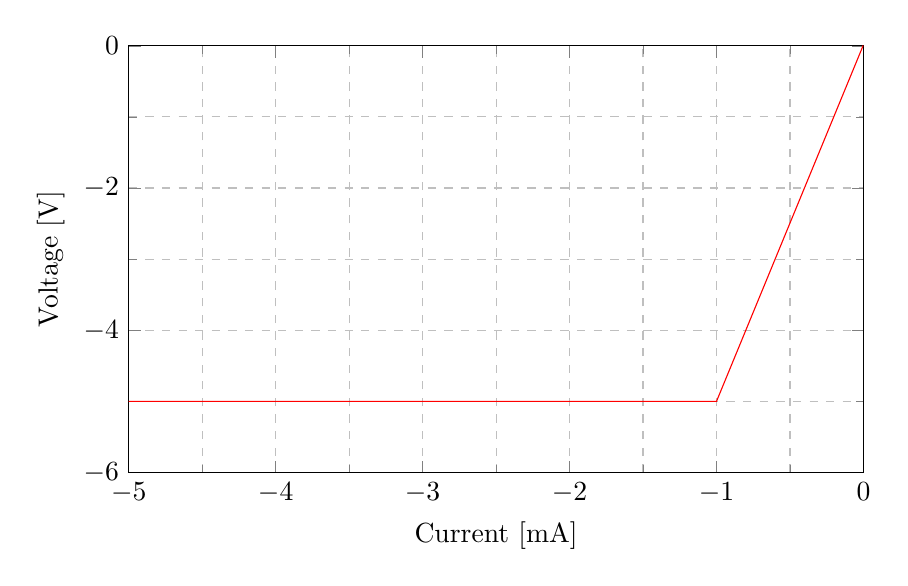
\begin{tikzpicture}

\begin{axis}[
    %title={Temperature dependence of CuSO$_4\cdot$5H$_2$O solubility},
    xlabel={Current [mA]},
    ylabel={Voltage [V]},
    height=7cm,
    width=0.9\textwidth,
    xmin=-5, xmax=0,
    ymin=-6, ymax=0,
    xtick={-5, -4, -3, -2, -1, 0},
    ytick={-6, -4, -2, 0},
    legend pos=south east,
    ymajorgrids=true,
    yminorgrids=true,
    xmajorgrids=true,
    xminorgrids=true,
    minor tick num=1,
    grid style=dashed,
]

\addplot[color=red]
  coordinates {
  (-5,-5.000208)
  (-4,-5.0002)
  (-3,-5.000109)
  (-2,-5.000188)
  (-1,-5.000329)
  (0,0.01416543)
};
  % \addlegendentry{$16\mu m$}


\end{axis}
\end{tikzpicture}

\caption{Reverse Current}
\label{fig:iv_reverse}
\end{center}
% \end{figure}

  \end{subfigure}
\caption{IV characteristics for forward and reverse currents on the LED.}
\label{fig:iv}
\end{figure}


Figure \ref{fig:iv} shows the forward and reverse current plots for this LED. The forward voltage turns on at $1.8V$ and increases to $2.5V$ at $300mA$. The reverse voltage doe not show a great deal. The voltage was limited to a range of $-5V$ to $5V$ and the first data point at $-1mA$ required more than $-5V$. As such, it shows a $-5V$ for all measured currents.
